% Syllabus Template from Arman Shokrollahi
% https://www.overleaf.com/latex/templates/syllabus-template-course-info/gbqbpcdgvxjs

\documentclass[11pt, letterpaper]{article}
%\usepackage{geometry}
\usepackage[inner=2cm,outer=2cm,top=2.5cm,bottom=2.5cm]{geometry}
\pagestyle{empty}
\usepackage{graphicx}
\usepackage{fancyhdr, lastpage, bbding, pmboxdraw}
\usepackage[usenames,dvipsnames]{color}
\definecolor{darkblue}{rgb}{0,0,.6}
\definecolor{darkred}{rgb}{.7,0,0}
\definecolor{darkgreen}{rgb}{0,.6,0}
\definecolor{red}{rgb}{.98,0,0}
\usepackage[colorlinks,pagebackref,pdfusetitle,urlcolor=darkblue,citecolor=darkblue,linkcolor=darkred,bookmarksnumbered,plainpages=false]{hyperref}
\renewcommand{\thefootnote}{\fnsymbol{footnote}}

\pagestyle{fancyplain}
\fancyhf{}
\lhead{ \fancyplain{}{Political Analysis in R} }
%\chead{ \fancyplain{}{} }
\rhead{ \fancyplain{}{Fall 2022} }%\today
%\rfoot{\fancyplain{}{page \thepage\ of \pageref{LastPage}}}
\fancyfoot[RO, LE] {page \thepage\ of \pageref{LastPage} }
\thispagestyle{plain}

%%%%%%%%%%%% LISTING %%%
\usepackage{listings}
\usepackage{caption}
\DeclareCaptionFont{white}{\color{white}}
\DeclareCaptionFormat{listing}{\colorbox{gray}{\parbox{\textwidth}{#1#2#3}}}
\captionsetup[lstlisting]{format=listing,labelfont=white,textfont=white}
\usepackage{verbatim} % used to display code
\usepackage{fancyvrb}
\usepackage{acronym}
\usepackage{amsthm}
\VerbatimFootnotes % Required, otherwise verbatim does not work in footnotes!



\definecolor{OliveGreen}{cmyk}{0.64,0,0.95,0.40}
\definecolor{CadetBlue}{cmyk}{0.62,0.57,0.23,0}
\definecolor{lightlightgray}{gray}{0.93}



\lstset{
%language=bash,                          % Code langugage
basicstyle=\ttfamily,                   % Code font, Examples: \footnotesize, \ttfamily
keywordstyle=\color{OliveGreen},        % Keywords font ('*' = uppercase)
commentstyle=\color{gray},              % Comments font
numbers=left,                           % Line nums position
numberstyle=\tiny,                      % Line-numbers fonts
stepnumber=1,                           % Step between two line-numbers
numbersep=5pt,                          % How far are line-numbers from code
backgroundcolor=\color{lightlightgray}, % Choose background color
frame=none,                             % A frame around the code
tabsize=2,                              % Default tab size
captionpos=t,                           % Caption-position = bottom
breaklines=true,                        % Automatic line breaking?
breakatwhitespace=false,                % Automatic breaks only at whitespace?
showspaces=false,                       % Dont make spaces visible
showtabs=false,                         % Dont make tabls visible
columns=flexible,                       % Column format
morekeywords={__global__, __device__},  % CUDA specific keywords
}

%%%%%%%%%%%%%%%%%%%%%%%%%%%%%%%%%%%%
\begin{document}
\begin{center}
{\Large \textsc{POLS 3230: Political Analysis in \texttt{R}}}
\end{center}
\begin{center}
{\large Fall 2022}
\end{center}

\begin{center}
\rule{6.5in}{0.4pt}
\begin{minipage}[t]{.96\textwidth}
\begin{tabular}{llcccll}
\textbf{Professor:} & Joe Ornstein & &  & \textbf{Time:} & MWF 11:30am -- 12:20pm \\
\textbf{Email:} &  \href{mailto:jornstein@uga.edu}{jornstein@uga.edu} & & & \textbf{Place:} & 101D Baldwin Hall\\
\textbf{Website:} & \href{https://joeornstein.github.io/pols-3230/}{https://joeornstein.github.io/pols-3230/} & & & &
\end{tabular}
\end{minipage}
\rule{6.5in}{0.4pt}
\end{center}
\vspace{.15cm}
\setlength{\unitlength}{1in}
\renewcommand{\arraystretch}{2}

\noindent In this course, you will learn the fundamentals of working with data using \texttt{R}, a programming language widely used among professional data scientists and academic researchers. You'll learn how to write code, explore new datasets, build visualizations, and think carefully about what conclusions you can and cannot draw from data.

\begin{figure}[h]
	\centering
	\href{https://xkcd.com/523/}{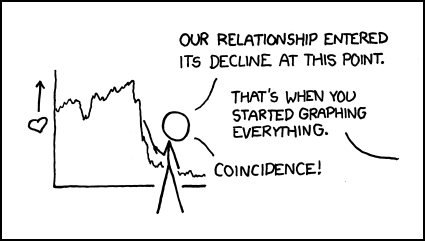
\includegraphics[width=0.6\textwidth]{img/decline.png}}
\end{figure}

%\begin{quotation}
%	\noindent``\textit{You can't really know anything if you just remember isolated facts. If the facts don't hang together on a latticework of theory, you don't have them in a usable form. You've got to have models in your head.}''\\
%	\\
%	--Charlie Munger (investor, vice chairman of Berkshire Hathaway)
%\end{quotation}

% \noindent 

\section*{Course Objectives}
%\vskip.15in
%\noindent\textbf{Course Objectives:}  
By the end of this course, you will be able to:
\begin{itemize}
	\item Write \texttt{R} scripts to import, tidy, and summarize datasets
	\item Create beautiful and informative data visualizations 
	\item Draw thoughtful conclusions from data
	\item Organize your work so that it is transparent and reproducible
%	\item Manipulate, wrangle, and clean datasets using the \texttt{R} programming language
%	\item Create beautiful data visualizations
%	\item Organize your work so that it is transparent and reproducible
%	\item Compute derivatives and solve systems of linear equations
%	\item Explain the properties of probability distributions and expected values
%	\item Perform hypothesis tests and fit models to data
\end{itemize}

\section*{Readings}
%I will expect you to read and annotate each assignment using \href{https://joeornstein.github.io/pols-3230/index.html#hypothesis}{Hypothesis}. 
Before each class session, I will assign a reading that walks you through a new \texttt{R} programming skill. All the readings will be available free online (including the books listed below!), but if you're the type of person who enjoys reading a hard copy, here is a list of books you can purchase:

\begin{itemize}
	\item \href{https://r4ds.had.co.nz/}{Wickham, H., \& Grolemund, G. (2016). \textit{R For Data Science: import, tidy, transform, visualize, and model data}. O'Reilly Media, Inc.}

	\item \href{https://clauswilke.com/dataviz/}{Wilke, Clause O. (2019). \textit{Fundamentals of Data Visualization: A Primer on Making Informative and Compelling Figures}}
	
	\item \href{https://socviz.co/}{Healy, Kieran (2018). \textit{Data Visualization: A Practical Introduction}. Princeton University Press.} 
	
	
\end{itemize} 

\section*{Assignments \& Grading}

Your course grade will be based on the following three assignments:

\begin{itemize}
	\item \textbf{Quizzes (30\%)}: There will be three in-class quizzes throughout the semester. I will give you a piece of code with a bunch of errors in it, and your job will be to fix the code so that it works. Points assigned based on how many errors you spot and fix. For Fall 2022, the quiz dates will be \textbf{September 21}, \textbf{October 26}, and \textbf{November 30}.
	\item \textbf{Team Projects (50\%):} Every day in class, we will work in teams of three students to answer a question about some dataset. Roughly once per week, your team will submit a report on your findings. Reports that are error-free, reproducible, thoughtful, and visually appealing will earn full credit.
	\item \textbf{Final Project (20\%):} To cap off the semester, you will create an original data visualization that explores a topic of your choice. Projects that are error-free, reproducible, thoughtful, and visually appealing will earn full credit, and my 3-5 favorites will receive a prize (your dataviz on a poster or coffee mug)! You can find a copy of the grading rubric \href{https://joeornstein.github.io/pols-3230/syllabus/POLS-3230-final-rubric.xlsx}{here}.
\end{itemize}

%\vskip.15in
%\noindent\textbf{Office Hours:} 
\section*{Office Hours and Email Policy}
I will be available for meetings every Wednesday before and after class, and you can sign up for 15 minute appointments \href{https://calendly.com/jornstein/15min}{here}. My office is Baldwin 304C, but if you prefer we can video chat through the class Discord server (I will send an invite link for the Discord during the first week of class).

If you send me an email, please allow me 24 hours to respond. Like many professors, my inbox is pretty overloaded. Also, I have small children, so it's my policy to not check email after 5pm or on weekends. 

\section*{Tentative Course Outline}

Moltke the Elder writes that no battle plan survives first contact with the enemy. The same is true for course outlines. We may need to be flexible and deviate from the plan if some topics require more or less attention, or we think of something completely unexpected that we want to do, and it takes up a few weeks. Caveats aside, here is what I have planned!

%\begin{center} 
%\begin{minipage}{6in}
%\begin{flushleft}
%Chapter 1 \dotfill ~$\approx$ 3 days \\
%{\color{darkgreen}{\Rectangle}} ~A little of probability theory and graph theory	
\subsubsection*{Week 1: Getting Started}
\textit{Pre-Class Survey, Overcoming Fear, Setting up Software}

\subsubsection*{Week 2: Intro To Data Visualization}
\textit{ggplot2, The Grammar of Graphics, Design Principles, Scatterplots}

\subsubsection*{Week 3: Fancier Data Visualizations}
\textit{Lines, Facets, Histograms, Distributions, Color, Themes}

\subsubsection*{Weeks 4-6: Tidying Messy Data}
\textit{Making New Variables, Grouping, Summarizing, Importing Filtering, Merging}

\subsubsection*{Week 7-8: Space}
\textit{Working with geographic data, Drawing maps}

\subsubsection*{Week 9-10: Time}
\textit{Working with dates, Difference-in-difference}

\subsubsection*{Weeks 11-12: Text As Data}
\textit{Strings, Twitter, Sentiment Analysis}

\subsubsection*{Week 13-15: Final Projects}
\textit{Work on whatever you want, then show it off}


%\end{flushleft}
%\end{minipage}
%\end{center}

%\vskip.15in
%\noindent\textbf{Important Dates:}
%\begin{center} \begin{minipage}{3.8in}
%\begin{flushleft}
%Midterm \#1      \dotfill ~\={A}b\={a}n 16, 1393  \\
%Midterm \#2      \dotfill ~\={A}zar 21, 1393  \\
%%Project Deadline \dotfill ~Month Day \\
%Final Exam       \dotfill ~Dey 18, 1393  \\
%\end{flushleft}
%\end{minipage}
%\end{center}



\subsection*{Academic Honesty}
Remember that when you joined the University of Georgia community, you agreed to abide by a code of conduct outlined in the academic honesty policy called \href{https://honesty.uga.edu/Academic-Honesty-Policy/Introduction/}{\textit{A Culture of Honesty}}. Team projects may, of course, be completed in teams, but you may not consult other people for help on the quizzes, and I expect your final projects to be your original work.

\subsection*{Mental Health and Wellness Resources}

\begin{itemize}
\item If you or someone you know needs assistance, you are encouraged to contact Student Care and Outreach in the Division of Student Affairs at 706-542-7774 or visit \href{https://sco.uga.edu}{https://sco.uga.edu}. They will help you navigate any difficult circumstances you may be facing by connecting you with the appropriate resources or services. 
\item UGA has several resources for a student seeking \href{https://www.uhs.uga.edu/bewelluga/bewelluga}{mental health services} or \href{https://www.uhs.uga.edu/info/emergencies}{crisis support}. 
\item If you need help managing stress anxiety, relationships, etc., please visit \href{https://www.uhs.uga.edu/bewelluga/bewelluga}{BeWellUGA} for a list of FREE workshops, classes, mentoring, and health coaching led by licensed clinicians and health educators in the University Health Center.
\item Additional resources can be accessed through the UGA App.
\end{itemize}



%%%%%% THE END 
\end{document} 